\documentclass[12pt]{article}

% fonts

\usepackage[scaled=0.92]{helvet}   % set Helvetica as the sans-serif font
\renewcommand{\rmdefault}{ptm}     % set Times as the default text font

\usepackage[T1]{fontenc}
\usepackage{amsmath}
\usepackage{amsfonts}

% page numbers
\usepackage{fancyhdr}
\fancypagestyle{newstyle}{
\fancyhf{} % clear all header and footer fields
\fancyfoot[R]{\vspace{0.1in} \small \thepage}
\renewcommand{\headrulewidth}{0pt}
\renewcommand{\footrulewidth}{0pt}}
\pagestyle{newstyle}

% geometry of the page
\usepackage[top=1in,
            bottom=1in,
            left=1in,
            right=1in]{geometry}

% paragraph spacing
\setlength{\parindent}{0pt}
\setlength{\parskip}{2ex plus 0.4ex minus 0.2ex}

% useful packages
\usepackage{natbib}
\usepackage{epsfig}
\usepackage{url}
\usepackage{bm}


\begin{document}

\large \textbf{Reader Report} \\
Reading: Title (Author, Year) \\
Name (Uni) \\
\today

\vspace{0.1in}

\normalsize

\section{Abstract}


\section{Introduction}
Venture capitalist and startup founders have been following two simple rules for decades - The success of startup relies on some irreplaceable talents of founders and the funding from large and prestigious VC funds.
To which extent are these success luck, and under which circumstances are these belief true remains an untold story even within the industry.

There are two widely believed hypothesis in the startup and venture capital industry. One is that changing a startup's CEO would be devastating, and the second is that being invested by large funds will more likely lead to success. While startup founders and investors held on to these believe, it is surprising that there are no research article or even commercial reports answering these two hypothesis. This is perhaps due to the lack of data and proper analytical tools for the private sector, letting alone the diversity of startups in recent year.

Given the availability of data in the private sector, we wish to test these two hypothesis using causal inference methods, and natural language processing tools.

We also encounter several difficulties. First, matching is inherently hard in the startup space. Perhaps because of the slow introduction of academic results into the business world, some researchers rely on TF-iDF. Second, it is impossible to do controlled experiments in the business world. Assigning a new CEO to a new company in an experimental, yet, what-if analysis is so important.

\section{Methodology}
\subsection{Data}
To this end, we used a free data set online which collected more than 190,000 startups in the US from 2003 to 2013 from Crunchbase. We filtered startups that have received at least one funding and were operating up until December 2013. In other words, we assume continuous operation during the period of our dataset and exclude any exogenous shocks such as acquisition or bankruptcy. This approach gave us around 26,000 startups.

For each of these startups, we obtain a time series of their founding rounds (i.e. Series A, B, C), including total money funded and the corresponding investors. These time series are discrete, with gaps close to one month, or as large as several years. To process the timeline of different startups in batches, we adopted a numerical sequencing of series to represent rounds of funding instead of raw timestamps, so that the founding timelines for different startups are aligned. 99\% of the startups only have 6 rounds of funding, so we restrict our attention to the first six rounds. After the data cleaning we have 4,372 startups.

Our goal is to study how changing leadership would cause changes to early-stage startups. The treatment is the record change of CEO or Founder. We obtain this data from the same dataset, and we convert the time of such leadership change to numerical sequencing. We observe that 96\% (4,215) companies did not change CEO, and the rest 157 startups changed leadership. For the purpose of this project, we assume that the treatment is binary, and there is no quantitatively better or worse change of the leadership.

We also downloaded the company's website page as an extra source of confounding. The reason for using text data is that startup data usually are not well-documented and well structured, as compared with public companies. This has historically contributed to the difficulty of analyzing startup ecosystem. This approach of using website data is similar to the approach of \cite{jorge}. In this paper, we first use Clearbit services to find the domain of the company from company names. Since startups usually change their business scope frequently, we use Wayback services to find the website html when the company was first founded. These website html files are transformed into pure texts for confounding purposes.

\begin{figure}
    \centering
    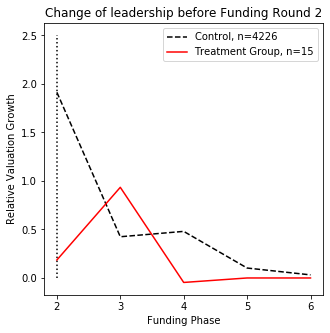
\includegraphics[width=.4\textwidth]{figures/r2.png}
    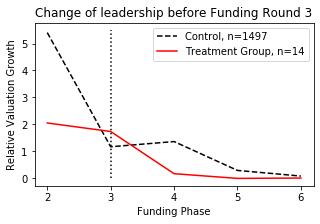
\includegraphics[width=.4\textwidth]{figures/r3.png}
    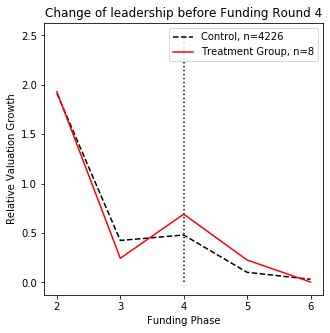
\includegraphics[width=.4\textwidth]{figures/r4.png}
    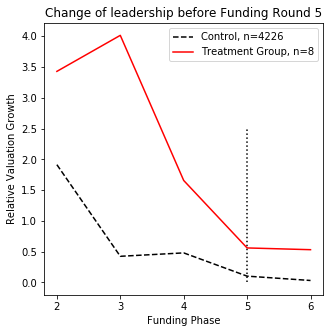
\includegraphics[width=.4\textwidth]{figures/r5.png}
    \caption{Change of leadership during the first 5 rounds of funding. The y-axis is the relative growth of the company. The x-axis is the funding phase. The intuition is that when the company was in its first two funding phase, it is unwise to switch leadership. When the startup shifts into later rounds of funding, changing leadership may create extra funding opportunities. }
    \label{fig:my_label}
\end{figure}


\subsection{Synthetic Control}

\end{document}

%%% Local Variables:
%%% mode: latex
%%% TeX-master: t
%%% End:
